\documentclass[11pt]{article}
\usepackage[utf8]{inputenc}
\usepackage[T1]{fontenc}
\usepackage{graphicx}
\usepackage[export]{adjustbox}
\graphicspath{ {./images/} }
\usepackage{amsmath}
\usepackage{amsfonts}
\usepackage{amssymb}
\usepackage[version=4]{mhchem}
\usepackage{stmaryrd}

\begin{document}
Cash-Funded CDOs Versus Synthetic CDOs

In addition to balance sheet versus arbitrage CDOs, another major distinction between CDOs is that of cash-funded versus synthetic. This distinction focuses on whether the SPV obtains the risk of the portfolio using actual (cash) holdings of assets or through derivative positions.

\begin{center}
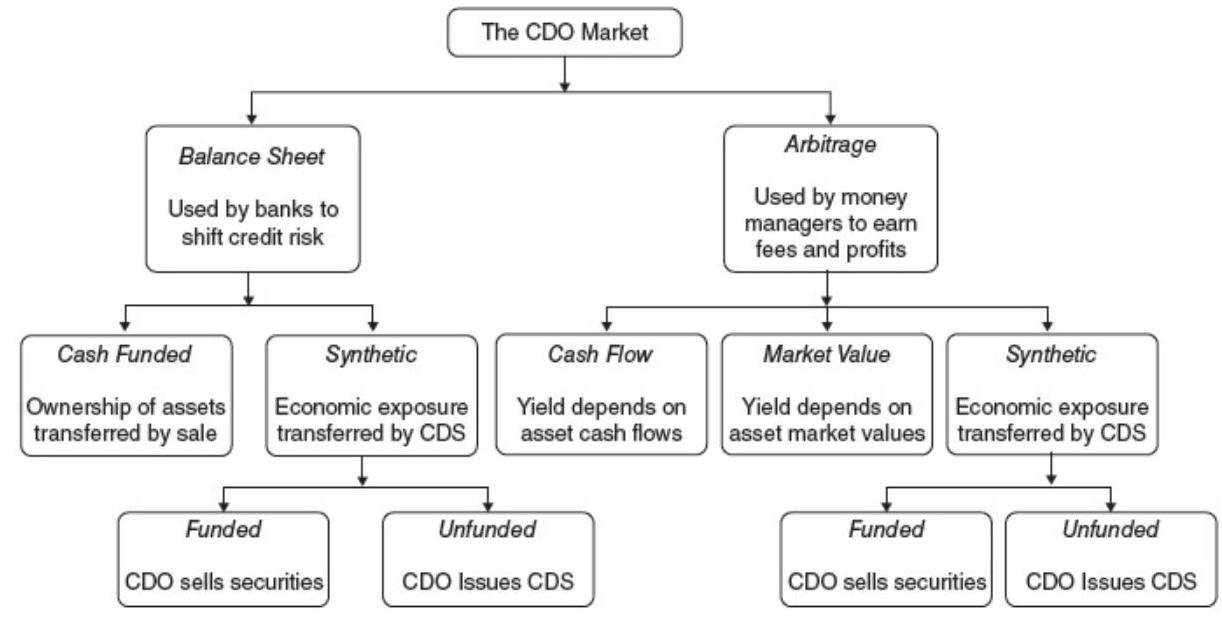
\includegraphics[max width=\textwidth]{2024_04_10_376aee6eb3365ddfffeeg-2}
\end{center}

\section*{Overview of Collateralized Debt Obligations}
Synthetic balance sheet CDOs differ from the cash-funded variety in several important ways. First, cash-funded CDOs are constructed with an actual sale and transfer of the loans or assets to the CDO trust. Ownership of the assets is transferred from the bank or other seller to the CDO trust in return for cash. In a synthetic CDO, however, the sponsoring bank or other institution transfers the risks and returns of a designated basket of loans or other assets via a credit derivative transaction, usually a credit default swap (CDS) or a total return swap. Therefore, the institution transfers the risk profile associated with its assets but does not give up the legal ownership of the assets and does not receive cash from selling assets. The above exhibit presents an overview of CDOs based on all of the distinctions detailed in this session.

\section*{Cash-Funded CDOs and Regulatory Capital}
A cash-funded CDO involves the actual purchase of the portfolio of securities serving as the collateral for the trust and to be held in the trust. In other words, physical ownership of the assets is acquired by the CDO. As is discussed in the next section, an analogous result can be obtained through derivatives in the case of a synthetic CDO. However, one advantage of a cash-funded CDO to a bank is that it can be used to completely replace risky assets with cash on the bank's balance sheet, rather than synthetically removing only the risk through derivatives.

There are several potential advantages to the financial institution in divesting risky assets using a cash-funded balance sheet CDO. Banks are required by regulators to maintain a particular level of capital, depending on the risk of their assets. Higher-risk assets require higher quantities of regulatory capital. Banks maintain regulatory capital by obtaining financing through common stock and other sources of financing that are considered to be more expensive than sources of capital that do not serve as regulatory capital, such as deposits. Reducing risk-based/regulatory capital is the most important motivation for a bank to form a CDO trust. Most major banks are required to maintain risk-based capital, such as $8 \%$ of the outstanding balance of commercial loans. Using a CDO trust to securitize and sell a portfolio of commercial loans can free up regulatory capital that must be committed to support the loan portfolio.

Sometimes the equity tranche of the CDO trust is unappealing to outside investors and cannot be sold. In this circumstance, the sponsoring bank may have to retain an equity or first-loss position in the CDO trust. If this is the case, the regulatory capital standards require the bank to maintain risk-based capital equal to its first-loss position. Thus, the bank needs to maintain $\$ 1$ in regulatory capital for each $\$ 1$ of ownership in an equity tranche.

There are numerous economic motivations to banks for issuing cash-funded balance sheet CDOs. By selling existing loans into a CDO trust, a lending institution receives cash proceeds from the sale of its loans to the CDO trust that can be used to originate additional commercial loans or to strengthen its balance sheet. With its cash in hand, the bank can reduce its overall balance sheet by paying down its liabilities. Additionally, the selling bank may be able to reduce its credit exposure to one industry or group of borrowers if the bank deems that its exposures are too high. The bank can preserve a relationship with a particular client by lending to a higher credit exposure than it would otherwise wish in order to maintain its relationship with its borrower, and then reduce its exposure through divesting some of the loans into a CDO.

\section*{Mechanics of Synthetic CDOs}
In a synthetic CDO, the CDO obtains risk exposure for the collateral pool through the use of a credit derivative, such as a total return swap or a CDS. Physical ownership of the underlying basket of securities is not transferred to the CDO, only the economic exposure. In effect, the CDO trust sells credit protection on a referenced basket of assets. For this protection and in the case of a CDS, the CDO receives income in the form of CDS payments from the credit protection buyer. The credit protection payments are then divided up among the CDO's investors into tranches, based on the seniority of the securities issued by the CDO.

In most cases, the CDO trust collects cash from the sale of the tranche securities and earns interest by investing the cash in low-risk collateral. Typically, the CDO invests the proceeds from issuing tranches in assets such as Treasury securities. The interest from the collateral combines with the CDS payments from the credit protection buyer to form a total return that should approximate the total return that would be received from physical ownership of the reference assets.

Synthetic CDOs are not limited to balance sheet CDOs. Synthetic arbitrage CDOs use derivatives to obtain desired risk exposure to reference assets similar to the exposure that could be attained through the cash purchase of the reference assets and avoid the need for any change in the legal ownership of the assets. Most synthetic balance sheet CDOs are constructed with a CDS. The CDO receives periodic payments from the credit protection buyer and must make a payment only if a trigger event such as a default occurs.

Synthetic arbitrage CDOs are used by asset management companies, insurance companies, and other investment shops with the intent of exploiting a mismatch between the higher income earned on the collateral and the lower cost of financing using the CDO tranches. Synthetic CDO structures are less administratively burdensome than cash-funded structures, particularly for attempting to transfer only a portion of a credit risk.

\section*{Comparison of Synthetic and Cash-Funded CDOs}
There are three major potential advantages to synthetic CDOs over cash-funded CDOs. First, a synthetic CDO is less burdensome than the transfer of assets required for a cash-funded CDO. Commercial loans may require borrower notification and consent before being transferred to the CDO trust. This can take time, increase administration costs, and lead to dissatisfaction on the part of the bank's loan customers. These problems are avoided if the risk is transferred by a CDS or a total return swap. Second, synthetic CDO trusts can be used to provide economic exposure to credit-risky assets that may be relatively scarce and difficult to acquire in the cash market. Last, synthetic CDO trusts can employ leverage by using derivatives to sell credit protection on assets of a size that is greater than the level of assets in the collateral pool.

Two difficulties posed by synthetic CDOs relative to cash-funded CDOs are potential exposure to counterparty risk and reduction in bankruptcy remoteness. First, consider the difference between a cash-funded CDO that purchases bonds from Bank XYZ and a synthetic CDO that enters a credit derivative with Bank XYZ. The exposure to counterparty risk emanates from the use of a credit derivative to obtain risk exposure rather than from the actual purchase of collateral assets with risk exposures. The CDO is exposed to the risk of bankruptcy by counterparties to the credit derivatives at the same time that the credit derivatives have positive market values. Second, a major advantage of CDOs is that their bankruptcy remoteness enhances the safety of tranches by reducing the chances that payments to tranche holders will be bogged down by the financial distress of one of the entities providing the collateral assets. When the CDO has direct ownership and physical possession of the credit risky collateral assets (cash funded), there are reduced potential legal entanglements than when the CDO has a relationship with an entity through one or more credit derivatives (synthetic).


\end{document}